\section{Experiment}
\subsection{Experimental Setting}
% \paragraph{Training Datasets.}
% XXX

\paragraph{Benchmarks.}
We evaluate \textsc{Seed} across three complementary forms of long-horizon agency. \textit{ALFWorld}~\citep{shridhar2021alfworld} casts household tasks as text-based embodied interaction, requiring an agent to interpret observations and execute extended action sequences. We consider six task families: \textit{Pick}, \textit{Look}, \textit{Clean}, \textit{Heat}, \textit{Cool}, and \textit{Pick2}. \textit{WebShop}~\citep{yao2022webshop} evaluates interactive web navigation, where an agent searches for products, inspects their attributes, and completes a purchase according to a natural-language request. We use the standard set of 128 test tasks. Finally, following the Search-R1 protocol~\citep{jin2025searchr1}, \textit{Search-based QA} requires an agent to gather evidence through search before answering questions from Natural Questions~\citep{kwiatkowski2019natural}, TriviaQA~\citep{joshi2017triviaqa}, PopQA~\citep{mallen2023popqa}, HotpotQA~\citep{yang2018hotpotqa}, 2WikiMultiHopQA~\citep{ho2020constructing}, MuSiQue~\citep{trivedi2022musique}, and Bamboogle~\citep{press2023measuring}. Together, these benchmarks cover embodied control, web-based decision making, and tool-augmented information seeking.

\vspace{-0.08in}

\paragraph{Baselines.}
We compare \textsc{Seed} with prompting, outcome-based RL, and distillation baselines. \textit{Vanilla} evaluates the instruction-tuned backbone without post-training, whereas \textit{Skill-Prompt} provides natural-language skills only in the evaluation context. \textit{GRPO}~\citep{shao2024deepseekmath} optimizes group-normalized trajectory rewards without auxiliary supervision. \textit{Skill-GRPO} additionally conditions the policy on skills during RL. We also include representative self-distillation and skill-distillation methods: \textit{OPSD}~\citep{zhao2026selfdistilledreasoner}, \textit{GRPO+OPSD}, \textit{Skill-SD}~\citep{wang2026skillsd}, \textit{RLSD}~\citep{yang2026rlsd}, and \textit{SDAR}~\citep{lu2026sdar}. These comparisons distinguish the effects of outcome optimization, access to skill context, and dense teacher-derived supervision. An asterisk denotes evaluation with skills; all other methods operate from the ordinary interaction history without privileged skill inputs at test time. We use matched backbones, rollout budgets, and training schedules for all reproduced post-training baselines.

\vspace{-0.08in}

\begin{table*}[ht!]
    \centering
    \caption{
        \textbf{Performance Comparison on the representative long-horizon benchmarks (ALFWorld, Search-based QA, and WebShop).}
        We report the success rate (\%) on ALFWorld, accuracy on Search-based QA, and task-completion score/success rate on WebShop. An asterisk (*) denotes validation with skills. The \sethlcolor{topcolor}\hl{\textbf{best}} and \sethlcolor{secondcolor}\hl{\mbox{\underline{second-best}}} results are highlighted.
    }
    \vspace{0.05in}
    \label{tab:main_results}
    \resizebox{\textwidth}{!}{%
    \begin{tabular}{l ccccccc cccccccc cc}
    \toprule
    & \multicolumn{7}{c}{\textbf{ALFWorld}}
    & \multicolumn{8}{c}{\textbf{Search-based QA}}
    & \multicolumn{2}{c}{\textbf{WebShop}} \\
    \cmidrule(lr){2-8}
    \cmidrule(lr){9-16}
    \cmidrule(lr){17-18}
    \textbf{Method}
    & \textbf{Pick} & \textbf{Look} & \textbf{Clean}
    & \textbf{Heat} & \textbf{Cool} & \textbf{Pick2} & \textbf{Avg}
    & \textbf{NQ} & \textbf{Triv} & \textbf{Pop}
    & \textbf{Hotp} & \textbf{2Wk} & \textbf{MuS}
    & \textbf{Bam} & \textbf{Avg}
    & \textbf{Score} & \textbf{Succ.} \\
    \midrule

    \rowcolor{gray!10}
    \multicolumn{18}{c}{\textit{Qwen2.5-3B-Instruct}} \\

    Vanilla
        & 44.4 & 11.1 & 6.2 & 15.4 & 28.6 & 12.5 & 21.9
        & 24.6 & 48.1 & 31.0 & 26.3 & 25.3 & 7.2 & 59.7 & 31.7
        & 6.7 & 0.8
        \\
    Skill-Prompt*
        & 51.7 & 66.7 & 48.4 & 0.0 & 4.3 & 10.0 & 28.9
        & 23.7 & 46.2 & 30.6 & 24.4 & 22.1 & 7.5 & 12.5 & 23.9
        & 0.2 & 0.8
        \\
    OPSD
        & 48.8 & 41.7 & 16.7 & 0.0 & 15.8 & 16.7 & 28.1
        & 0.1 & 0.1 & 0.1 & 0.0 & 0.0 & 0.0 & 0.0 & 0.0
        & 11.3 & 3.1
        \\
    GRPO
        & 91.2 & 62.5 & \cellcolor{secondcolor}\underline{96.2}
        & 61.9 & 65.0 & 47.4 & 75.0
        & 39.3 & 60.6 & 41.1 & 37.4 & 34.6 & 15.4 & 26.4 & 36.4
        & 79.8 & 63.3
        \\
    Skill-GRPO
        & 88.9 & 71.4 & 58.8 & 70.6 & 40.7 & 29.2 & 60.2
        & 43.5 & 58.8 & 43.0 & 36.8 & 32.2 & 11.7 & 12.5 & 34.1
        & 77.3 & 60.9
        \\
    Skill-GRPO*
        & 94.3 & 57.1 & \cellcolor{topcolor}\textbf{100.0}
        & 66.7 & \cellcolor{secondcolor}\underline{73.1}
        & 57.1 & 80.5
        & 44.3 & 59.6 & 44.3 & 39.0 & 36.1 & 14.5 & 14.9 & 36.1
        & 76.3 & 66.4
        \\
    GRPO+OPSD
        & \cellcolor{topcolor}\textbf{100.0}
        & \cellcolor{secondcolor}\underline{82.4}
        & 85.7
        & \cellcolor{secondcolor}\underline{75.0}
        & 70.0 & 60.0 & 81.2
        & \cellcolor{topcolor}\textbf{44.9}
        & \cellcolor{secondcolor}\underline{61.2}
        & \cellcolor{secondcolor}\underline{45.2}
        & \cellcolor{secondcolor}\underline{40.4}
        & 38.5 & 16.0 & 66.1
        & \cellcolor{secondcolor}\underline{44.6}
        & 77.8 & 66.4
        \\
    Skill-SD
        & 88.2 & 50.0 & \cellcolor{secondcolor}\underline{96.2}
        & 52.4 & 65.0 & 57.9 & 73.4
        & 44.4 & 60.4 & 44.0 & 39.5
        & \cellcolor{secondcolor}\underline{40.4}
        & 15.4 & 64.9 & 44.1
        & 75.9 & 64.0
        \\
    RLSD
        & 87.9 & 75.0 & 90.9
        & \cellcolor{secondcolor}\underline{75.0}
        & \cellcolor{secondcolor}\underline{73.1}
        & 68.4 & 79.7
        & 41.5 & 58.6 & 42.3
        & \cellcolor{secondcolor}\underline{40.4}
        & 40.2
        & \cellcolor{secondcolor}\underline{16.8}
        & \cellcolor{secondcolor}\underline{66.9}
        & 43.8
        & 84.4 & 66.4
        \\
    SDAR
        & \cellcolor{secondcolor}\underline{97.1}
        & 62.5
        & \cellcolor{topcolor}\textbf{100.0}
        & 61.9
        & \cellcolor{topcolor}\textbf{75.0}
        & \cellcolor{topcolor}\textbf{84.2}
        & \cellcolor{secondcolor}\underline{84.4}
        & \cellcolor{secondcolor}\underline{44.8}
        & 58.1 & 44.3 & 38.6 & 36.2 & 15.7 & 66.1 & 43.4
        & \cellcolor{secondcolor}\underline{85.0}
        & \cellcolor{secondcolor}\underline{68.0}
        \\
    \textbf{\textsc{Seed} (Ours)}
        & \cellcolor{topcolor}\textbf{100.0}
        & \cellcolor{topcolor}\textbf{100.0}
        & \cellcolor{topcolor}\textbf{100.0}
        & \cellcolor{topcolor}\textbf{100.0}
        & 70.6
        & \cellcolor{secondcolor}\underline{80.0}
        & \cellcolor{topcolor}\textbf{91.8}
        & 44.3
        & \cellcolor{topcolor}\textbf{61.9}
        & \cellcolor{topcolor}\textbf{47.2}
        & \cellcolor{topcolor}\textbf{41.0}
        & \cellcolor{topcolor}\textbf{42.0}
        & \cellcolor{topcolor}\textbf{16.9}
        & \cellcolor{topcolor}\textbf{67.7}
        & \cellcolor{topcolor}\textbf{45.7}
        & \cellcolor{topcolor}\textbf{88.5}
        & \cellcolor{topcolor}\textbf{78.9}
        \\

    \midrule

    \rowcolor{gray!10}
    \multicolumn{18}{c}{\textit{Qwen2.5-7B-Instruct}} \\

    Vanilla
        & 36.1 & 22.2 & 3.1 & 0.0 & 0.0 & 0.0 & 12.5
        & 25.2 & 50.8 & 29.5 & 29.0 & 29.0 & 10.4 & 63.7 & 33.9
        & 5.9 & 1.6
        \\
    Skill-Prompt*
        & 51.7 & 50.0 & 32.3 & 5.3 & 4.3 & 0.0 & 23.4
        & 30.9 & 52.1 & 32.7 & 32.7 & 27.9 & 12.7 & 66.1 & 36.4
        & 1.7 & 0.8
        \\
    OPSD
        & 50.0 & 60.0 & 22.7 & 21.4 & 17.6 & 9.5 & 32.8
        & 8.8 & 8.6 & 17.5 & 2.5 & 4.2 & 0.5 & 1.2 & 6.2
        & 4.5 & 2.3
        \\
    GRPO
        & 91.2 & 87.5 & 96.2 & 81.0 & 65.0 & 57.9 & 81.2
        & 45.1 & 63.7 & 44.0 & 43.6 & 43.2 & 16.8 & 37.6 & 42.0
        & 80.9 & 72.6
        \\
    Skill-GRPO
        & 88.5 & 66.7 & 65.2 & 61.1 & 57.7 & 73.1 & 69.5
        & 45.2 & 63.7 & 45.7 & 43.1 & 43.3 & 19.6 & 21.4 & 40.3
        & 80.4 & 71.9
        \\
    Skill-GRPO*
        & \cellcolor{topcolor}\textbf{100.0}
        & 83.3
        & \cellcolor{secondcolor}\underline{96.4}
        & 83.3 & 75.0
        & \cellcolor{secondcolor}\underline{78.9}
        & \cellcolor{secondcolor}\underline{88.3}
        & 44.8 & 63.0 & 45.1 & 43.7 & 43.7
        & \cellcolor{secondcolor}\underline{20.5}
        & \cellcolor{secondcolor}\underline{71.4}
        & 47.5
        & 87.0
        & \cellcolor{secondcolor}\underline{81.2}
        \\
    GRPO+OPSD
        & 91.4 & 61.5
        & \cellcolor{topcolor}\textbf{100.0}
        & \cellcolor{secondcolor}\underline{87.5}
        & 76.5 & 52.2 & 80.4
        & \cellcolor{topcolor}\textbf{47.3}
        & \cellcolor{secondcolor}\underline{64.5}
        & 46.9 & 43.8 & 39.3 & 18.0 & 69.4 & 47.0
        & 86.8 & 76.5
        \\
    Skill-SD
        & 93.9
        & \cellcolor{secondcolor}\underline{93.8}
        & 90.9
        & \cellcolor{topcolor}\textbf{100.0}
        & 69.2 & 68.4 & 85.1
        & \cellcolor{secondcolor}\underline{47.1}
        & \cellcolor{secondcolor}\underline{64.5}
        & \cellcolor{secondcolor}\underline{47.8}
        & 44.2 & 42.1 & 20.2 & 69.0 & 47.8
        & 86.1 & 76.5
        \\
    RLSD
        & \cellcolor{topcolor}\textbf{100.0}
        & 87.5 & 92.3 & 58.8
        & \cellcolor{secondcolor}\underline{80.0}
        & 65.2 & 82.0
        & 46.8 & 63.0 & 44.4
        & \cellcolor{topcolor}\textbf{45.5}
        & \cellcolor{topcolor}\textbf{48.9}
        & \cellcolor{topcolor}\textbf{21.5}
        & \cellcolor{topcolor}\textbf{73.0}
        & \cellcolor{topcolor}\textbf{49.0}
        & 87.4 & 77.3
        \\
    SDAR
        & \cellcolor{secondcolor}\underline{94.7}
        & 75.0
        & \cellcolor{topcolor}\textbf{100.0}
        & 86.7 & 68.2
        & \cellcolor{secondcolor}\underline{78.9}
        & 85.9
        & 46.3 & 63.5
        & \cellcolor{topcolor}\textbf{48.2}
        & 43.8
        & \cellcolor{secondcolor}\underline{48.4}
        & 19.6
        & \cellcolor{topcolor}\textbf{73.0}
        & \cellcolor{topcolor}\textbf{49.0}
        & \cellcolor{secondcolor}\underline{89.4}
        & \cellcolor{topcolor}\textbf{82.8}
        \\
    \textbf{\textsc{Seed} (Ours)}
        & \cellcolor{topcolor}\textbf{100.0}
        & \cellcolor{topcolor}\textbf{100.0}
        & 96.3 & 80.0
        & \cellcolor{topcolor}\textbf{100.0}
        & \cellcolor{topcolor}\textbf{100.0}
        & \cellcolor{topcolor}\textbf{96.1}
        & 47.0
        & \cellcolor{topcolor}\textbf{64.9}
        & \cellcolor{secondcolor}\underline{47.8}
        & \cellcolor{secondcolor}\underline{45.2}
        & 45.3 & 20.1 & 70.2
        & \cellcolor{secondcolor}\underline{48.6}
        & \cellcolor{topcolor}\textbf{89.7}
        & 78.1
        \\

    \midrule

    \rowcolor{gray!10}
    \multicolumn{18}{c}{\textit{Qwen3-1.7B-Instruct}} \\

    Vanilla
        & 25.0 & 22.2 & 3.1 & 0.0 & 21.4 & 4.2 & 12.5
        & 29.4 & 46.9 & 37.0 & 23.5 & 19.6 & 6.4 & 10.5 & 24.8
        & 46.5 & 4.7
        \\
    Skill-Prompt*
        & 10.3 & 50.0 & 16.1 & 0.0 & 0.0 & 5.0 & 9.4
        & 29.4 & 46.5 & 36.2 & 22.9 & 20.8 & 4.3 & 10.1 & 24.3
        & 23.0 & 2.3
        \\
    OPSD
        & 26.3 & 33.3 & 9.1 & 0.0 & 4.5 & 5.3 & 14.1
        & 4.2 & 8.3 & 4.6 & 6.6 & 15.3 & 0.7 & 1.2 & 5.8
        & 47.4 & 9.3
        \\
    GRPO
        & 71.1 & 41.7 & 36.4 & 40.0 & 31.8 & 31.6 & 46.1
        & 40.0
        & \cellcolor{topcolor}\textbf{58.9}
        & 43.5 & 35.4 & 30.3 & 12.0 & 65.7 & 40.8
        & 67.3 & 38.3
        \\
    Skill-GRPO
        & 27.6
        & \cellcolor{secondcolor}\underline{54.5}
        & 22.7 & 27.3 & 0.0 & 19.2 & 21.1
        & 39.2
        & \cellcolor{secondcolor}\underline{58.6}
        & 43.9 & 35.2 & 28.2 & 11.5
        & \cellcolor{secondcolor}\underline{66.1}
        & 40.4
        & 73.4 & 46.1
        \\
    Skill-GRPO*
        & 31.4 & 42.9 & 51.9 & 8.3 & 11.5 & 7.1 & 28.1
        & 38.0 & 58.4 & 43.9 & 36.3 & 29.0 & 12.5
        & \cellcolor{topcolor}\textbf{66.9}
        & 40.7
        & 80.4 & 50.0
        \\
    GRPO+OPSD
        & 38.2 & 50.0 & 30.8 & 28.6 & 30.0 & 21.1 & 32.0
        & \cellcolor{secondcolor}\underline{40.7}
        & \cellcolor{topcolor}\textbf{58.9}
        & 45.0
        & \cellcolor{topcolor}\textbf{37.0}
        & 34.6
        & \cellcolor{topcolor}\textbf{13.3}
        & 65.7
        & \cellcolor{topcolor}\textbf{42.2}
        & 70.7 & 38.3
        \\
    Skill-SD
        & 52.9 & 37.5 & 69.2
        & \cellcolor{secondcolor}\underline{42.9}
        & \cellcolor{secondcolor}\underline{60.0}
        & \cellcolor{secondcolor}\underline{36.8}
        & 52.3
        & 39.1 & 57.5
        & \cellcolor{secondcolor}\underline{45.4}
        & 34.8 & 34.1 & 10.7 & 64.1 & 40.8
        & \cellcolor{secondcolor}\underline{81.8}
        & 53.9
        \\
    RLSD
        & 50.0 & 37.5 & 61.5 & 19.0 & 50.0 & 21.1 & 42.2
        & 38.6 & 57.3 & 43.0 & 34.5 & 34.1 & 11.5 & 65.3 & 40.6
        & 74.0 & 50.8
        \\
    SDAR
        & \cellcolor{secondcolor}\underline{73.5}
        & 25.0
        & \cellcolor{secondcolor}\underline{76.9}
        & 33.3 & 40.0
        & \cellcolor{secondcolor}\underline{36.8}
        & \cellcolor{secondcolor}\underline{53.9}
        & 39.7
        & \cellcolor{topcolor}\textbf{58.9}
        & 45.3 & 35.9
        & \cellcolor{topcolor}\textbf{35.5}
        & \cellcolor{secondcolor}\underline{12.6}
        & 65.3
        & \cellcolor{secondcolor}\underline{41.9}
        & 76.8
        & \cellcolor{secondcolor}\underline{58.6}
        \\
    \textbf{\textsc{Seed} (Ours)}
        & \cellcolor{topcolor}\textbf{97.6}
        & \cellcolor{topcolor}\textbf{100.0}
        & \cellcolor{topcolor}\textbf{100.0}
        & \cellcolor{topcolor}\textbf{80.0}
        & \cellcolor{topcolor}\textbf{84.2}
        & \cellcolor{topcolor}\textbf{90.0}
        & \cellcolor{topcolor}\textbf{92.0}
        & \cellcolor{topcolor}\textbf{42.0}
        & \cellcolor{topcolor}\textbf{58.9}
        & \cellcolor{topcolor}\textbf{47.1}
        & \cellcolor{secondcolor}\underline{36.9}
        & \cellcolor{secondcolor}\underline{35.2}
        & 10.6 & 64.9
        & \cellcolor{topcolor}\textbf{42.2}
        & \cellcolor{topcolor}\textbf{87.1}
        & \cellcolor{topcolor}\textbf{77.3}
        \\

    \bottomrule
    \end{tabular}
    }
\end{table*}

\paragraph{Evaluation Metrics.}
For ALFWorld, we report the success rate for each task family and their unweighted macro-average. For WebShop, we follow the environment protocol and report both the mean normalized task-completion score and the exact success rate. For Search-based QA, we compute answer accuracy separately on all seven subsets and report their unweighted macro-average. All metrics are expressed as percentages, and higher values indicate better performance.
\vspace{-0.08in}

\paragraph{Implementation Details.}
We use Qwen2.5-3B-Instruct and Qwen2.5-7B-Instruct~\citep{yang2024qwen25}, as well as Qwen3-1.7B-Instruct~\citep{yang2025qwen3}, as our backbone models.
\textit{SFT stage:}
For each backbone, we sample $M=180$ training tasks and collect $K_0=8$ rollout trajectories per task, resulting in 1,440 completed trajectories.
We then query GLM-5.2~\citep{zai2026glm52} as an external trajectory analyzer to extract hindsight skills from these trajectories.
After lightweight format validation, the retained trajectory--skill pairs are used to fine-tune the corresponding backbone for three epochs.
\textit{RL stage:}
The resulting SFT checkpoint initializes both the policy and the synchronized trajectory analyzer.
We train each model for 150 policy updates, using a batch size of 16 on ALFWorld and WebShop and 128 on Search-based QA.
The rollout group size is set to $N=8$ for all benchmarks.
Additional details on SFT data construction, skill annotation, optimization, and hyperparameter settings are provided in Appendix~\ref{app:implementation_details}.

\subsection{Main Results}\label{subsec32_main_results}
Table~\ref{tab:main_results} reports the results across different model scales and agentic domains. Three findings emerge:

\textbf{\textsc{Seed} consistently outperforms outcome-only RL through dense supervision.} Relative to GRPO, \textsc{Seed} improves the ALFWorld macro-average by 14.9-45.9 points, Search-based QA by 1.4-9.3 points, the WebShop task-completion score by 8.7-19.8 points, and the success rate by 5.5-39.0 points across the three backbones. Compared with Skill-GRPO, which conditions exploration on natural-language skills but still broadcasts a single terminal-reward-derived advantage to all valid tokens, \textsc{Seed} further improves the ALFWorld average by 26.6-70.9 points, Search-based QA by 1.8-11.6 points, the WebShop score by 9.3-13.7 points, and the success rate by 6.2-31.2 points. These consistent improvements over both GRPO and Skill-GRPO demonstrate that dense token-level hindsight supervision provides more effective credit assignment than outcome-only optimization, leading to substantially stronger performance across long-horizon agentic tasks.

\begin{figure}[t]
    \centering
    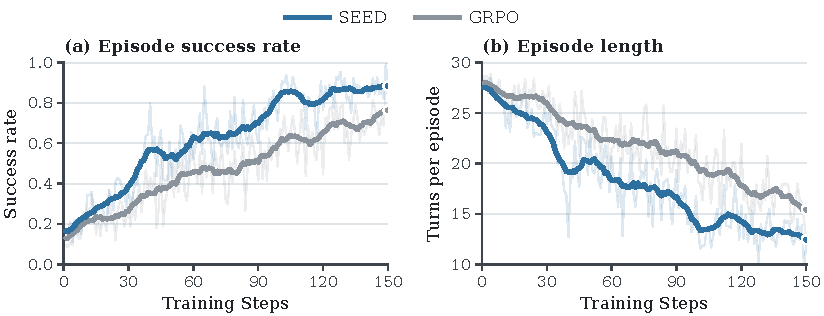
\includegraphics[width=\linewidth]{figures/training_dynamics.pdf}
    \caption{
        \textbf{Training dynamics on ALFWorld.}
        We compare \textsc{Seed} and GRPO using Qwen2.5-3B-Instruct as the backbone. Translucent curves show raw measurements, while solid curves show 13-point centered moving averages.
    }
    \label{fig:training_dynamics}
\end{figure}

\textbf{Internalizing skills is substantially more effective than inserted prompts.}
Skill-Prompt, which provides skills only during evaluation, underperforms \textsc{Seed} on every aggregate metric across all three backbones. \textsc{Seed} also exceeds Skill-GRPO* in 11 of the 12 aggregate comparisons, despite using no skill context during evaluation. These results indicate that hindsight skills are more effective when distilled into the policy than when supplied as additional context at inference time.

\textbf{Self-evolving hindsight distillation is stronger than static self-distillation.}
Across the static distillation baselines, \textsc{Seed} achieves the best or tied best result in 10 of the 12 aggregate comparisons. The advantage is clearest on ALFWorld, where \textsc{Seed} outperforms the strongest static baseline by 7.4 points with Qwen2.5-3B, 10.2 points with Qwen2.5-7B, and 38.1 points with Qwen3-1.7B. This pattern supports the benefit of synchronizing the analyzer with the latest policy, so hindsight supervision adapts to the trajectories and failure modes encountered during training.

\subsection{Training Dynamics}
Figure~\ref{fig:training_dynamics} compares the optimization dynamics of \textsc{Seed} and GRPO on ALFWorld. The success-rate curves diverge early: by training step 40, \textsc{Seed} reaches roughly 57\% while GRPO remains near 35\%, and the advantage persists thereafter. \textsc{Seed} also reduces the mean episode length more quickly, from approximately 28 turns to 13, compared with about 16 turns for GRPO at the end of training. Because shorter trajectories coincide with higher success, this reduction reflects more efficient task execution rather than premature termination. Together, these trends indicate that \textsc{Seed} improves task completion and interaction efficiency by reducing unproductive exploration and learning more direct solution strategies.


\subsection{Sample Efficiency}\label{subsec33_efficiency_analysis}
Figure~\ref{fig:sample_efficiency_line} shows that \textsc{Seed} consistently outperforms GRPO across all data fractions and can match or surpass the performance of GRPO trained with substantially more data. Using only 60\% of the training instances, \textsc{Seed} achieves a score of 80.7, exceeding the 75.0 obtained by GRPO with the full training set. Similarly, with 40\% of the data, \textsc{Seed} reaches 58.9, closely matching GRPO trained with twice as much data, which achieves 58.6 at the 80\% setting. These results demonstrate that \textsc{Seed} extracts more informative and effective supervision from each completed trajectory than outcome-only RL based solely on terminal rewards. Detailed results are provided in Appendix~\ref{app:sample_efficiency}.

\subsection{Cross-Domain Generalization}\label{subsec34_cross_domain_generalization}
We further evaluate the 3B checkpoint trained with \textsc{Seed} and GRPO on the ALFWorld unseen split. As shown in Figure~\ref{fig:generalization_bar}, \textsc{Seed} increases the macro-average success rate from 70.9 to 86.2, outperforming GRPO by 15.3 points and achieving better performance in five of the six task families. The largest improvements are observed on \textit{Heat} (+35.0), \textit{Look} (+18.3), and \textit{Pick} (+16.5). These results indicate that the policy trained with \textsc{Seed} acquires reusable behavioral strategies that transfer effectively to unseen environments, rather than merely memorizing the training trajectories. Detailed results are provided in Appendix~\ref{app:ood_generalization}.

\begin{figure}[ht!]
\centering
\begin{minipage}[t]{0.48\linewidth}
    \centering
    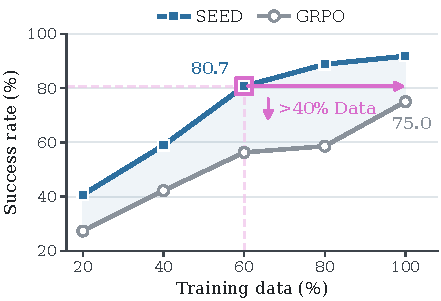
\includegraphics[width=\linewidth]{figures/sample_efficiency_line.pdf}
    \vspace{-0.15in}
    \caption{
        \textbf{Sample efficiency analysis.} \textsc{Seed} consistently outperforms GRPO across different data fraction settings and surpasses full-data GRPO using only 60\% of the training data.
    }
    \label{fig:sample_efficiency_line}
\end{minipage}
\hfill
\begin{minipage}[t]{0.48\linewidth}
    \centering
    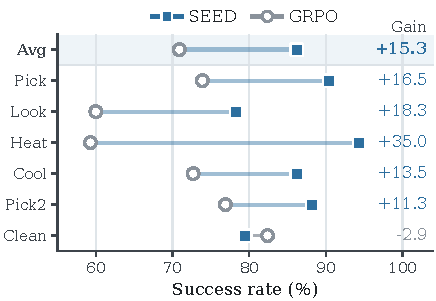
\includegraphics[width=\linewidth]{figures/generalization_bar.pdf}
    \vspace{-0.15in}
    \caption{
        \textbf{Cross-domain generalizability on ALFWorld Unseen.} \textsc{Seed} generally outperforms GRPO across unseen task types, demonstrating stronger cross-domain generalizability.
    }
    \label{fig:generalization_bar}
\end{minipage}
\end{figure}

\begin{table}[ht!]
\centering
\caption{
    \textbf{Ablation Results.}
    We report \textsc{Seed} performance and its ablated variants on ALFWorld.
}
\vspace{0.05in}
\label{tab:ablation_seed}
\small
\renewcommand{\arraystretch}{1.08}
\begin{tabular}{lccccccc}
\toprule
& \multicolumn{7}{c}{\textbf{ALFWorld}} \\
\cmidrule(lr){2-8}
\textbf{Method}
& \textbf{Pick}
& \textbf{Look}
& \textbf{Clean}
& \textbf{Heat}
& \textbf{Cool}
& \textbf{Pick2}
& \textbf{Avg.} \\
\midrule
% GRPO
%     & 91.2
%     & 62.5
%     & 96.2
%     & 61.9
%     & 65.0
%     & 47.4
%     & 75.0
%     \\
\rowcolor{gray!10}
\textsc{Seed}
    & \textbf{100.0}
    & \textbf{100.0}
    & \textbf{100.0}
    & \textbf{100.0}
    & 70.6
    & 80.0
    & \textbf{91.8}
    \\
\;\;\;w/o Hindsight Skill SFT
    & 97.6
    & 81.8
    & 92.6
    & 90.0
    & \textbf{84.2}
    & 70.0
    & 86.0
    \\
\;\;\;w/o Self-Evolving OPD
    & 93.3
    & 70.0
    & 96.9
    & 84.6
    & 76.9
    & \textbf{100.0}
    & 87.0
    \\
\;\;\;w/o On-Policy Skill
    & 97.1
    & 62.5
    & \textbf{100.0}
    & 61.9
    & 75.0
    & 84.2
    & 84.4
    \\
\bottomrule
\end{tabular}
\end{table}

\subsection{Ablation Studies and Analysis}
Table~\ref{tab:ablation_seed} evaluates the contribution of the three core components of \textsc{Seed}.

\textbf{The impact of hindsight-skill SFT.}
Removing hindsight-skill SFT decreases the ALFWorld average from 91.8 to 86.0, corresponding to a 5.8-point drop. This result shows that equipping the actor and analyzer with an initial trajectory-analysis capability provides an important foundation for the subsequent self-evolving training process.

\textbf{The impact of self-evolving OPD.}
Removing self-evolving OPD reduces the average performance to 87.0, a decrease of 4.8 points. This indicates that the one-time skill supervision introduced during SFT is insufficient on its own, and that continuously distilling supervision from newly collected trajectories is necessary to keep pace with the evolving policy.

\textbf{The impact of on-policy skills.}
Replacing on-policy skills with skills from a static offline library leads to the largest performance degradation, lowering the average to 84.4 by 7.4 points. This finding highlights the importance of deriving guidance from the current policy's own trajectories, as such skills better reflect its evolving behaviors and failure modes.

\paragraph{Qualitative Analysis. }
Figure~\ref{fig:case_comparison} presents a representative example of the behavioral differences between GRPO and \textsc{Seed}. GRPO visits the target receptacle before locating the required object, interacts with irrelevant objects, and repeatedly explores unproductive locations until reaching the step limit. In contrast, \textsc{Seed} follows a more coherent and goal-directed trajectory: it searches plausible storage locations, identifies the candle on the second shelf, and completes the task with the correct placement action. The more direct trajectory exhibited by \textsc{Seed} is consistent with its stronger performance and higher interaction efficiency reported in the preceding experiments.


\begin{figure}[ht!]
    \centering
    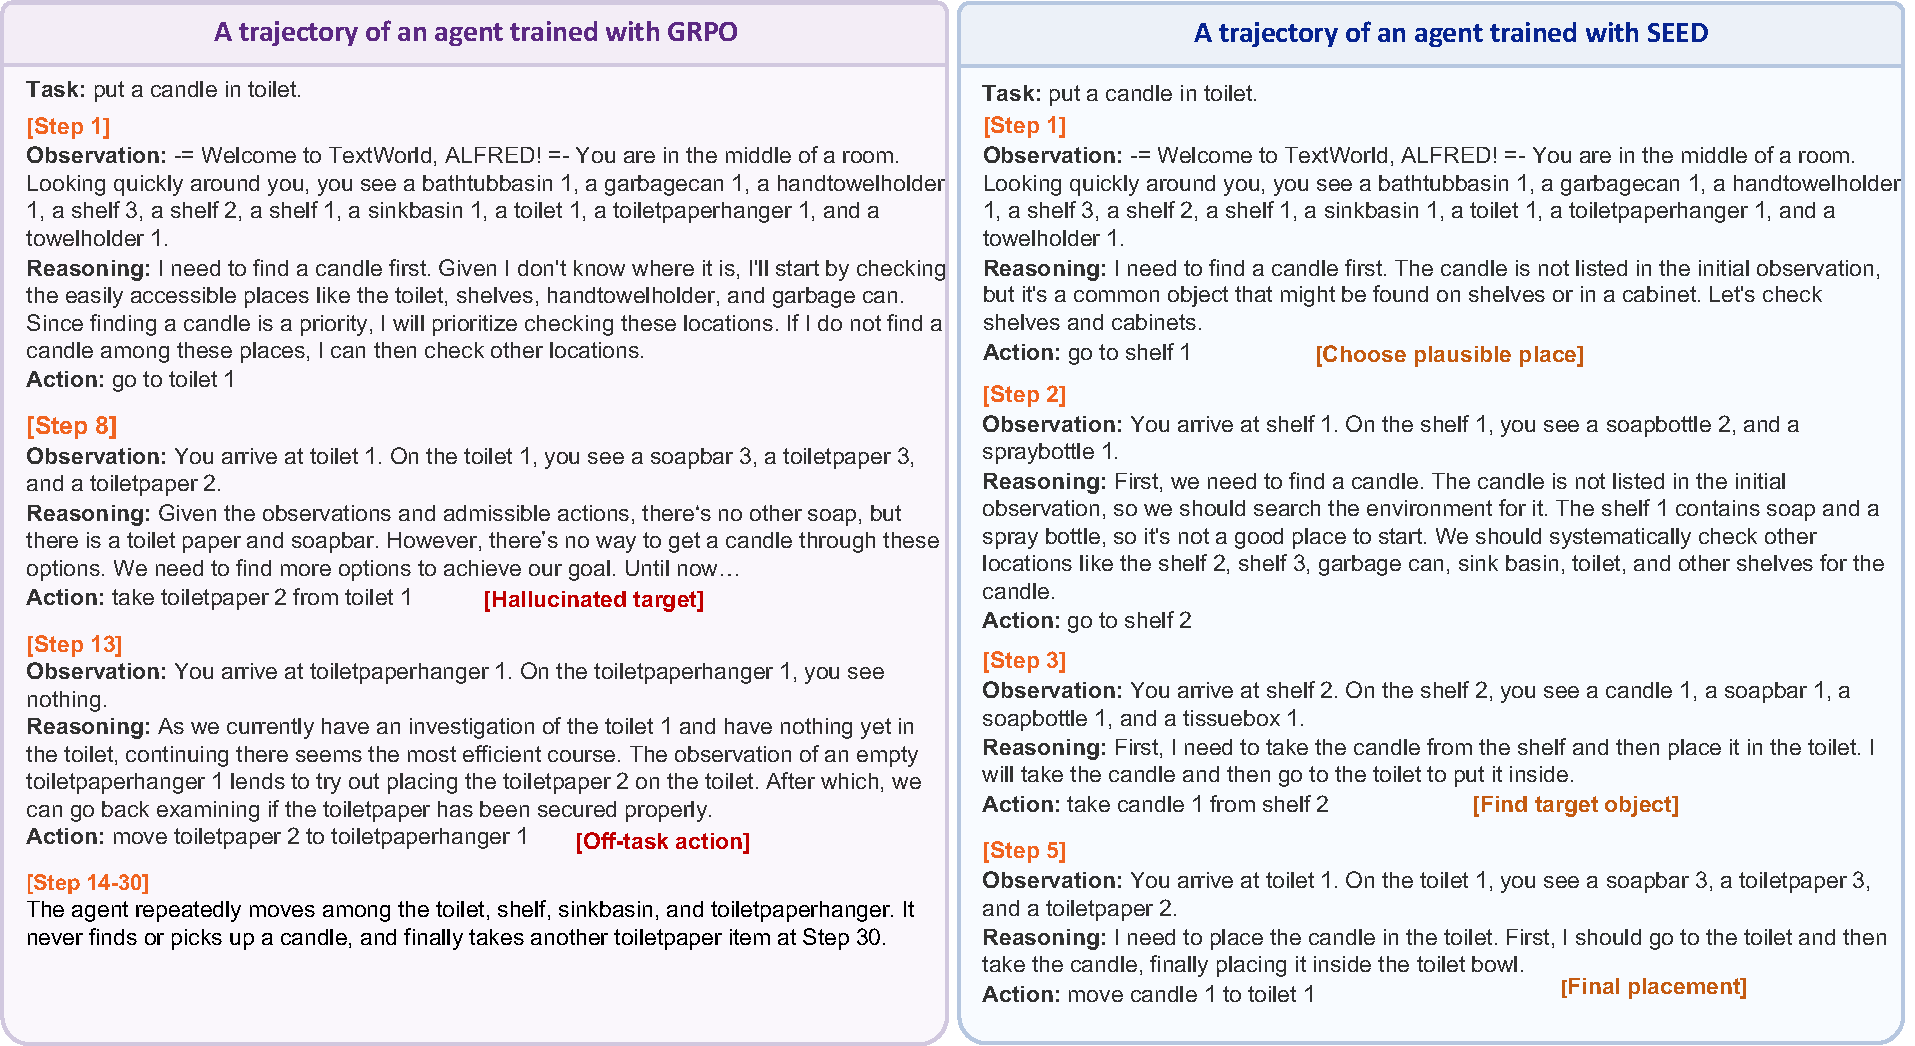
\includegraphics[width=\linewidth]{figures/SEED_case.pdf}
    \caption{
        \textbf{Qualitative comparison on ALFWorld.}
        For the task “put a candle in toilet,” the GRPO-
        trained agent searches the target receptacle before locating the candle, takes an irrelevant toilet-paper
        item, and then enters an off-task loop. In contrast, SEED systematically checks plausible shelves,
        finds the candle, and completes the required placement in five steps.
    }
    \label{fig:case_comparison}
\end{figure}
